\documentclass[a4paper, 11pt,oneside]{article}
\usepackage[
  top=1.5cm,
  bottom=1cm,
  left=2cm,
  right=1.5cm,
  headheight=25.22153pt, % as per the warning by fancyhdr
  includehead,includefoot,
  heightrounded, % to avoid spurious underfull messages
]{geometry} 

\usepackage{pdflscape}
\usepackage[T1]{fontenc}
\usepackage{microtype}
\usepackage{fancyhdr}
\usepackage{fancyvrb}
\usepackage{lipsum}
\usepackage{url}
\usepackage{listings}
\usepackage{lastpage}
\usepackage{enumitem}
\usepackage{datetime}
\usepackage{amsthm}
\usepackage{graphicx}
\usepackage{hyperref}
\usepackage{caption}
\usepackage[newfloat]{minted}
\usepackage{float}

\captionsetup[listing]{position=bottom}

\settimeformat{hhmmsstime}
\yyyymmdddate

\pagestyle{fancy}
\fancyhf{} % clear all fields

\pagestyle{fancy}
\lhead{CMSC 132: Computer Architecture \\ First Semester 2020-2021}
\rhead{Institute of Computer Science \\ University of the 
Philippines Los Banos}
\rfoot{$\copyright$JACHermocilla (CC NC-BY-SA 4.0)}
%\cfoot{Enjoy!:)}
\cfoot{\thepage\ of \pageref{LastPage}}
\lfoot{Revision: \today\ \currenttime}
%\rfoot{https://jachermocilla.org/teaching/125}
\renewcommand{\headrulewidth}{0.4pt}
\renewcommand{\footrulewidth}{0.4pt}

\begin{document}

\begin{center}
	{\LARGE \textbf{Instruction Set Architecture Design and Implementation}}
\end{center}

\section*{Learning Outcomes}
   At the end of this lab, you should be able to:
   \begin{enumerate}[itemsep=0pt,parsep=0pt]
   	   \item understand and modify a simple ISA;
       \item write a simple assembler
   \end{enumerate}   
\tableofcontents

\section{Resources}
\begin{itemize}
	\item Video: \href{https://youtu.be/CzyXb_T-xgU}{https://youtu.be/CzyXb\_T-xgU}.
	\item Source Codes: \href{https://git.io/JU3al}{https://git.io/JU3al}
	\item Online VHDL Tool: \href{https://www.edaplayground.com/home}
	{https://www.edaplayground.com/home}
\end{itemize}	

\section{Discussion}
The \textbf{processor(CPU)} is composed of the \textbf{datapath} and 
\textbf{control}. In the previous labs, you learned that combinational and 
sequential circuit elements are used as building blocks to create the 
functional components of the datapath and control. Examples of these functional 
elements include the \textbf{ALU, Register File, Program Counter, and Memory}. 
You also learned that a \textbf{clock} drives the execution and control is 
implemented using a \textbf{finite state machine} for 
\textbf{fetch-decode-execute cycle}. One question that we can answer next is: 
\textit{How do we program the CPU?}


\subsection{Instruction Set Architecture}
Instruction Set Architecture (ISA) is an \textbf{abstraction} between the 
hardware and the lowest-level software. It includes anything programmers need 
to know to make a binary machine language program work correctly. Typically it  
documents the set of instructions that can be performed by the 
processor, number and name of available registers, memory 
addressing modes, I/O, interrupt processing, etc.

ISA allows computer designers to talk about functions indepedently from the 
hardware that performs them. This abstact interface enables many 
implementations (aka \textbf{microarchitectures}) of varying costs and 
performance to run identical software.

Examples of ISA include the \textbf{IA-32} and \textbf{x86-64} which are 
commonly used in desktop and laptops. Intel implements these ISA in their Intel 
Core i5 product as \textbf{8th Generation aka as Kaby Lake Refresh}. AMD also 
implements these ISA in the Ryzen 5000 as \textbf{4th Gen aka Zen 3}. There are 
other implementations(aka generations) that vary in their performance 
characteristics.

For mobile devices, a popular ISA is the \textbf{ARMv8 A64}. MediaTek uses 
ARM's \textbf{Cortex-A73} and \textbf{Cortex-A53} implementations in their 
Octa-core Helio P70. Qualcomm also uses the same implementations in their Kryo 
240 processor for Snapdragon SoC.

\subsection{Application Binary Interface}
Application Binary Interface (ABI) is a combination of the basic instruction 
set and the operating system interface provided for application programmers. 

For general-purpose use such a desktops and laptops, programming a processor 
using only the basic instruction set is inefficient. Thus, operating systems 
perform an important role in the management and efficient use of hardware 
resources in addition to making it easier for users to use a computer. 

ABI describes function-calling conventions, parameter passing, sizes of 
C data types, executable file formats (ELF, PE). Examples are the IA-32 and 
\textbf{x86-64 System V ABI} which is used in Linux and other Unix-type 
operating systems. In Windows, it uses its own \textbf{x64 ABI}.

\subsection{ISA Taxonomy}
We can categorize ISAs based on where operands in instructions are stored.
\textbf{Stack-based} ISAs uses a stack(LIFO) where operations are performed on 
the operands on the top of the stack. In \textbf{accumulatr-based} ISAs, one 
register is designated as accumulator and its use in operations is implied. 
Modern ISAs are \textbf{general purpose} where operands are explicitly named in 
the instruction. Operations can be register-to-register, register-to-memory, 
or memory-to-register.

\subsection{Considerations in ISA Design}
\begin{itemize}
\item \textit{Types/Class of instructions(Operations in the instruction set)} - 
arithmetic/logic, data movement, branching/control flow, I/O, etc.
\item \textit{Types and sizes of operands} - 8, 16, 32, 64, 128, floating point
\item \textit{Addressing modes} - register, direct, indirect, immediate, etc.
\item \textit{Addressing memory} - byte-addressable, word-addressable
\item \textit{Encoding and Instruction Formats} - opcode field, addresses 
field, mode 
field
\item \textit{Compiler-related issues} - optimization features
\end{itemize}

\subsection{Example Instruction Formats}
Figure \ref{fig:x86-64} and Figure \ref{fig:armv8}  are the instruction formats 
for x86-64 and ARMv8, taken from their documentation manuals. The x86-64 format 
is more complex than that of the ARMv8 with variable widths in terms of number 
of bits for the opcode.

\begin{figure}[H]
	\begin{center}
	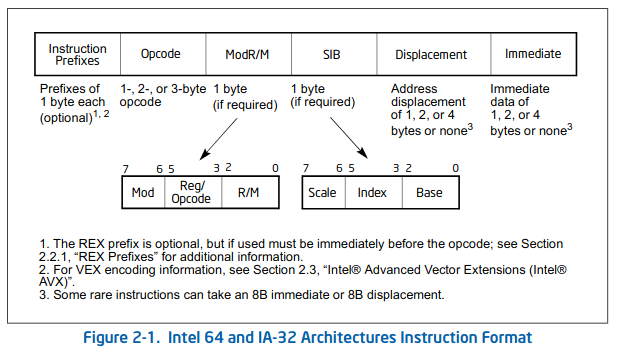
\includegraphics[width=4in]{x86-64.png}
	\caption{x86-64 Instruction Format (CISC).}
	\label{fig:x86-64} 
	\end{center}
\end{figure}

\begin{figure}[H]
	\begin{center}
	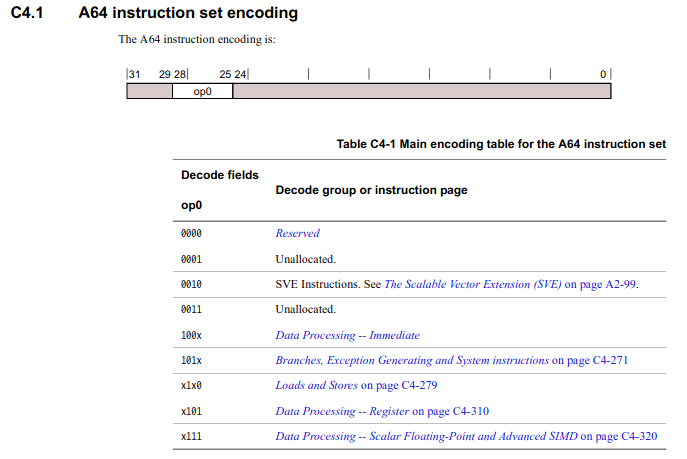
\includegraphics[width=4in]{armv8.png}
	\caption{ARMv8 Instruction Format (RISC).}
	\label{fig:armv8} 
	\end{center}
\end{figure}

\subsection{The Optimal Machine Architecture (TOMA) ISA}
Let us look at the design of a simple ISA called TOMA.

\subsubsection{Features}
\begin{itemize}
\item Four 8-bit registers named \mintinline{asm}{$s0, $s1, $s2, $s3} when 
used in assembly code
\item Instruction memory (IM) is 8 bytes(8x8), address line is 3 bits
\item Three-bit Program Counter (PC)
\item Single-cycle - completes instruction execution in one clock cycle
\item Supports the following instructions: \mintinline{asm}{and, add, sub, 
addi}
\item No data memory, thus has no load and store instructions
\item No control transfer instructions
\end{itemize}

\subsubsection{Instruction Format}
The size of an instruction in TOMA is 8 bits divided into the configuration 
shown in Figure \ref{fig:ins_format}.

\begin{figure}[H]
	\begin{center}
	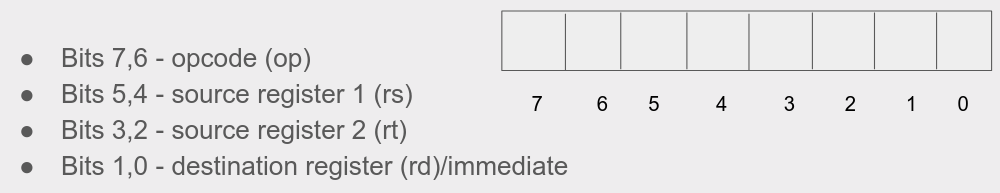
\includegraphics[width=5in]{ins_format.png}
	\caption{TOMA instruction format.}
	\label{fig:ins_format} 
	\end{center}
\end{figure}

\subsubsection{Supported Instructions}
\begin{listing}[H]
\caption{Supported Instructions in TOMA.}
\label{code:instructions}
\begin{minted}[frame=single,framesep=10pt]{vhdl}
and : rd <= rs AND rt           (op=00)
add : rd <= rs + rt             (op=01)
sub : rd <= rs -  rt            (op=10)
addi : rs <= rt + immediate     (op=11)
\end{minted}
\end{listing}


\subsubsection{Example assembly code and machine code}

\begin{listing}[H]
\caption{Example assembly code and machine code.}
\label{code:assembly}
\begin{minted}[frame=single,framesep=10pt]{nasm}
addi $s0, $s0, 2         ; 11000010b, 0xC2
addi $s1, $s1, 1         ; 11010101b, 0xD5
addi $s2, $s2, 3         ; 11101011b, 0xEB
add $s3, $s0, $s1        ; 01000111b, 0x47
sub $s0, $s2, $s3        ; 10101100b, 0xAC
\end{minted}
\end{listing}

The syntax for the assembly language isn shown in Listing \ref{code:assembly}.

\begin{listing}[H]
\caption{Example assembly code and machine code.}
\label{code:assembly}

\begin{minted}[frame=single,framesep=10pt]{nasm}
<instruction> <dst>, <src1>, <src2/imm>
\end{minted}
\end{listing}

\subsection{REDHORSE 500: An implementation of TOMA}
Given the TOMA ISA, let us implement the ISA and call it REDHORSE 500. We will 
use VHDL for the implementation.

\subsubsection{Processor}
The interface to the processor is shown in the code below which has one input 
and two outputs. 
\begin{minted}[frame=single,framesep=10pt]{vhdl}
ENTITY Processor IS 
    PORT
    (
        clk :  IN  STD_LOGIC;
        current_instruction :  OUT  STD_LOGIC_VECTOR(2 DOWNTO 0);
        value :  OUT  STD_LOGIC_VECTOR(7 DOWNTO 0)
    );
END Processor;
\end{minted}




\begin{landscape}
\thispagestyle{plain}
\begin{figure}[H]
	\begin{center}
	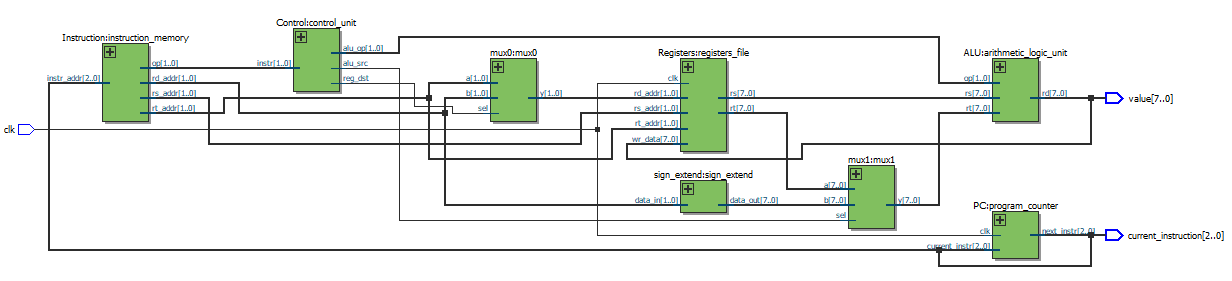
\includegraphics[width=10.5in]{redhorse500.png}
	\caption{REDHORSE 500.}
	\label{fig:redhorse500} 
	\end{center}
\end{figure}
\end{landscape}
%%[width=10in]



\begin{minted}[frame=single,framesep=10pt]{vhdl}
LIBRARY ieee;
USE ieee.std_logic_1164.all;
ENTITY clocker_tb IS
END clocker_tb;
ARCHITECTURE behavior OF clocker_tb IS
   --100Mhz
   CONSTANT frequency: integer := 100e6; 
   CONSTANT period : time := 1000 ms / frequency;
   SIGNAL clk : std_logic := '0';
BEGIN 
   clk <= not clk after period / 2;
   -- do some stuff here using clk as input
END ARCHITECTURE;
\end{minted}

\section{Summary}
In this lab, you learned some of the sequential elements that are useful in the 
design of a processor as well as the importance of clocks. We also showed the
design and implementation of a simple traffic light system using finite state 
machines since a simple truth table is not enough to characterize a sequential 
system. 

You should now be able to tell whether a functional component of a datapath and 
control is composed of a combinational or sequential element.

\section{Learning Activities}
Download the source codes for this lab then try experimenting by adding more 
test cases in the testbenches. Submit a PDF document that shows screenshots of 
your modifications and runs. 

\section{Self-Assessment Questions}
\begin{enumerate}
\item What is the main purpose of clocks in sequential circuits?
\item What is the difference between a clocked latch and a flip-flop?
\item Why can't a multiplexer be used in RAM?
\item Why is SRAM more expensive than DRAM?
\item If my CPU is clocked at 800 MHz, what is the period?
\end{enumerate}


\section{Deliverable}
Your final deliverable for this lab is implement the RAM in Figure 
 \ref{fig:sram3}. Submit the VHDL code including a testbench as well as images 
of the waveforms. NOTE: Enable lines should be connected to the output of the 
decoder and the rightmost Din in the figure should be Din[0].

\section{Further Reading}
\begin{itemize}
\item 
\href{https://www.doulos.com/knowhow/vhdl/simple-ram-model/}
{https://www.doulos.com/knowhow/vhdl/simple-ram-model/}
\end{itemize}


%\begin{thebibliography}{9}
%\end{thebibliography}

\bibliographystyle{unsrt}
\bibliography{toma}
\nocite{*}

\end{document}